\documentclass{article}
\usepackage{graphicx} % Required for inserting images
\usepackage{amssymb}
\usepackage{amsmath}
\usepackage{amsfonts}
\usepackage{extarrows}
\usepackage{soul}
\tolerance=1
\emergencystretch=\maxdimen
\hyphenpenalty=10000
\hbadness=10000
\let\oldemptyset\emptyset
\usepackage[T1]{fontenc}

\author{Amnézic}
\date{2023}
\title{Résumé du cours de THLR}

\begin{document}
\maketitle
\begin{figure}[h]
    \centering
    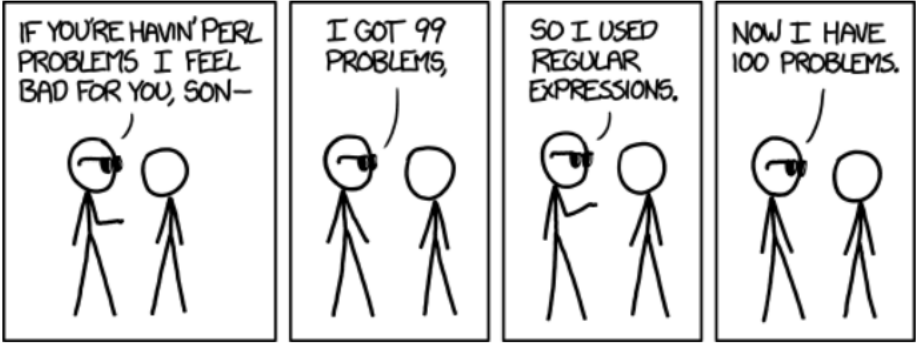
\includegraphics[scale=0.3]{Image1.png}
\end{figure}
\newpage
\tableofcontents
\newpage

\section{Introduction}
Un langage est un ensemble de séquences d'objets élémentaires auxquels on associe un sens. Chaque langage dépend d'un ensemble limité de symboles élémentaires.\newline

\subsection{Définitions}
\textbf{Alphabet:}\newline
Un alphabet est un ensemble $\Sigma$ de symboles. On appelle les éléments de $\Sigma$ des lettres. Un alphabet ne peut pas contenir plusieurs fois un même élément.\newline

\textbf{Mot :}
\begin{itemize}
    \item Un mot $w$ dans un alphabet $\Sigma$ est une séquence finie (possiblement vide) de lettres. Le mot vide est noté $\varepsilon$.
    \item L'ensemble $\Sigma^{*}$ est l'ensemble des tous les mots sur $\Sigma$ et l'ensemble\newline$\Sigma^{+}$ = $\Sigma^{*}$ $\symbol{92}$ $\{\varepsilon\}$\newline
\end{itemize}

\textbf{Langage :}
\begin{itemize}
    \item Un langage $L$ sur un alphabet $\Sigma$ est un ensemble de mots de $\Sigma$*
    \item L peut être fini ou infini
    \item $L \subseteq \Sigma^{*}$ = $L$ est un sous-ensemble de l'ensemble de tous les mots\newline
\end{itemize}
\subsection{Opérations sur les mots :}
Pour ces calculs, il faut obligatoirement donné un alphabet de référence. Les opérations \guillemotleft mathématiques \guillemotright :
\begin{itemize}
    \item longueur d'un mot : la longueur d'un mot $w$ sur un alphabet $\Sigma$, notée $|w|$, est égale au nombre de lettres ($|\varepsilon|$ = 0)
    \item occurrences d'un mot : l'occurrence d'un mot $w$ sur un alphabet $\Sigma$ et une lettre $a \in \Sigma$, $|w|_{a}$ correspond au nombre d'occurrences de $a$ dans $w$
    \item concaténation : soient deux mots $w_{1}$ = $a_{1}$...$a_{n}$ et $w_{2}$ = $b_{1}$...$b_{m}$, on définit leur concaténation $w_{1} \bullet w_{2}$ = $a_{1}$...$a_{n}b_{1}$...$b_{m}$
    \item propriétés de la concaténation :
    \begin{itemize}
        \item $|w_{1} + w_{2}|$ = $|w_{1}|$ + $|w_{2}|$
        \item $\varepsilon \bullet w_{1}$ = $w_{1} \bullet \varepsilon$ = $w_{1}$
        \item $w_{1} \bullet (w_{2} \bullet w_{3})$ = $(w_{1} \bullet w_{2}) \bullet w_{3} \Rightarrow$ associative
        \item pas commutative
    \end{itemize}
    \item exponentiation d'un mot : $w^{k}$ = $w$...$w$ k fois ($w^{0}$ = $\varepsilon$)
\end{itemize}
Les mots dérivés : (soient w, x, y, z d'un alphabet $\Sigma$)
\begin{itemize}
    \item x est un préfixe de w si w = x $\bullet$ y
    \item z est un suffixe de w si w = y $\bullet$ z
    \item y est un facteur de w si w = x $\bullet$ y $\bullet$ z
    \item $\varepsilon$ appartient à Pref(w), Suff(w) et Fact(w)
    \item inversion d'un mot : soit w = $w_{1}$...$w_{n}$ alors son miroir, noté $w^{R}$, est $w_{n}$...$w_{1}$ (si $w$ = $w_{R}$, alors w est un palindrome)
\end{itemize}
\subsection{Distance d'un mot}
\textbf{Définition :}\newline
La distance d'édition $d_{e}$($w_{1}$,$w_{2}$) entre deux mots $w_{1}$ et $w_{2}$ $\in$ $\Sigma^{*}$ est égal au nombre minimal d'insertions et de suppressions lettre par lettre nécessaire pour passer de $w_{1}$ à $w_{2}$.

Soit $E$ un ensemble, une fonction d : $E^{2} \rightarrow$ $R_{+}$ renvoie la distance si elle vérifie les propriétés suivantes ($\forall$x, y, z$\in$ $E$):
\begin{itemize}
    \item séparation : d$_{e}(x,y)$ = 0 $\Longleftrightarrow$ x = y
    \item symétrie : d$_{e}$(x,y) = d$_{e}$(y,x)
    \item inégalité triangulaire : d$_{e}$(x,y) + d$_{e}$(y,z) $\geq$ d$_{e}$(x,z)
\end{itemize}
\section{Langages décidables}
\subsection{Définition :}
Un langage $L$ sur un alphabet $\Sigma$ est dit décidable ou récursif s'il existe un algorithme $A$ tel que, pour tout $w \in \Sigma^{*}$
\begin{itemize}
    \item if $w \in L$, alors A(w) renvoie true
    \item sinon, A(w) renvoie false
\end{itemize}
Un langage $L$ sur un alphabet $\Sigma$ est dit semi-décidable ou récursivement énumérable s'il existe un algorithme $A$ tel que, pour tout $w \in \Sigma^{*}$.
\begin{itemize}
    \item si $w \in L$, alors A(w) renvoie true
    \item si $w \notin L$, alors A(w) revoie false \textbf{ou ne finit jamais}
\end{itemize}
Note : Si un langage L est récursif, alors il est récursivement énumérable (l'inverse est faux).\newpage
On peut voir les langages comme des ensembles en probabilités, il partage d'ailleurs certaines propriétés:
\begin{itemize}
    \item $\overline{(\overline{A})}$ = A
    \item A $\cup$ $\overline{A}$ = $\Sigma^{*}$
    \item $\overline{(A \cup B)}$ = $\overline{A}\cap\overline{B}$
    \item $\overline{(A \cap B)}$ = $\overline{A} \cup \overline{B}$
    \item A $\cap$ (B$\cup$C) = (A$\cup$B)$\cap$(A$\cup$C)
    \item A $\cup$ (B$\cap$C) = (A$\cup$B)$\cap$(A$\cup$C)
\end{itemize}
\subsection{Préfixes, facteurs et suffixes}
Soit L un langage sur $\Sigma$, le préfixe d'un langage est l'ensemble de tous les mots qui sont les préfixes d'au moins un mot de L. De manière plus formelle on le définit comme ceci :
\begin{quote}
    \item Pref(L) = \{ w $|$ x $\in$ L, w $\in$ Pref(x) \} 
\end{quote}
Note : cette définition s'applique aussi aux facteurs et aux suffixes
\subsection{Étoile de Kleen :}
Pour tout langage L, on a les propriétés suivantes :
\begin{itemize}
    \item $\varepsilon \in L^{*}$, même si $\varepsilon \notin L$
    \item $\varepsilon \in L^{+}$ ssi $\varepsilon \in L$
    \item $\emptyset^{*}$ = \{$\varepsilon$\}
    \item $\Sigma^{*}$ = $\Sigma^{*}$
\end{itemize}
\newpage
\section{Expressions régulières}
\subsection{Les bases}
Les symboles des motifs de langages :
\begin{itemize}
    \item + : ou $\rightarrow$ a + b = a ou b
    \item "(" and ")" : but uniquement syntaxique
    \item (x)* : répétition finie (potentiellement 0 fois) de x
    \item pour écrire un ensemble assez instinctif, on peut remplacer les ... par - \newline $\rightarrow$ \{A,...,Z\} = [A-Z]
    \item $x^{?}$ = $x$ + $\varepsilon$ : la lettre $x$ est optionnelle
    \item $x^{+}$ = $xx^{*}$ : $x$ est présent au moins une fois
\end{itemize}
\subsection{Définition}
\textbf{Syntaxe d'expression régulière}\newline
L'ensemble Reg$_{\Sigma}$ sur un alphabet finie $\Sigma$ qui ne contient pas les symboles réservés (ceux utilisés plus haut) est défini inductively par :
\begin{itemize}
    \item atomes : $\emptyset$, $\varepsilon$ et $a$ ($\forall a \in \Sigma$) sont des expressions régulières
    \item règles : si $e_{1}$ et $e_{2}$ sont des expressions régulières, alors $e_{1}$ + $e_{2}$, $e_{1}e_{2}$ et $e_{1}^{*}$ aussi
    \item profondeur : (pas compris)
\end{itemize}
Note: ces règles ne s'appliquent pas pour les intersections et les unions
\begin{figure}[h]
    \centering
    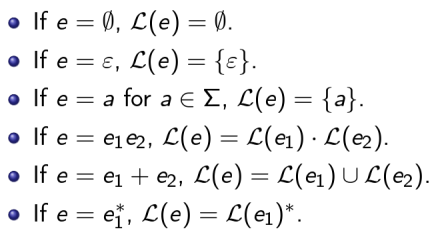
\includegraphics[scale=0.25]{Image2.png}
    \caption{Sémantique d'expressions régulières}
\end{figure}

\newpage
\textbf{Langages rationnels}\newline
L'ensemble $Rat_{\Sigma}$ des langages définis sur un alphabet $\Sigma$ est défini ainsi :
\begin{center}
    \item Rat = \{L $\subseteq \Sigma^{*} | \exists$ e $\in Reg_{\Sigma}$, L = $\mathfrak{L}$(e)\}
\end{center}
\begin{itemize}
    \item Un langage rationnel est un langage décidable.
    \item Un même langage peut être décrit par une infinité d'expressions régulières. Si $\mathfrak{L}$($e_{1}$) = $\mathfrak{L}$($e_{2}$) $\Longleftrightarrow$ $e_{1}$ $\equiv$ $e_{2}$
\end{itemize}
\begin{figure}[h]
    \centering
    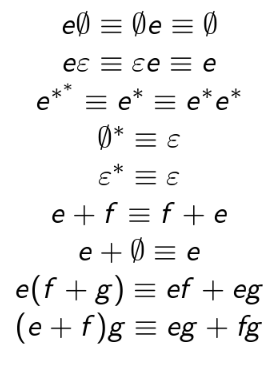
\includegraphics[scale=0.3]{Image3.png}
    \caption{Équivalences d'expressions régulières}
\end{figure}
\newpage
\section{Automates}
\subsection{Définition}
Un automate fini $A(Q,\Sigma,\delta,I,F)$ est composé de 5 éléments :
\begin{itemize}
    \item un ensemble fini $Q$ d'états : un état est un noeud du graphe
    \item un alphabet fini $\Sigma$
    \item un ensemble de transitions $\delta$ $\subseteq$ $Q \times \Sigma \times Q$ : une transition est un triplé, et $\delta$ est un ensemble de triplés
    \item un ensemble d'états initiaux $I$
    \item un ensemble d'états finaux/terminaux/acceptants $F$
\end{itemize}
Un automate $A$ accepte un mot $w \in \Sigma$ s'il existe un chemin depuis un état initial jusqu'à un état final nommé par $w$.\newline
Le langage $L$($A$) = \{w $\in \Sigma^{*} | A$ accepte w\} d'un automate $A$ est l'ensemble des tous les mots dans $\Sigma^{*}$ accepté par $A$. On dit que $\mathfrak{L}$($A$) est reconnu par $A$.\newline

\subsection{Propriétés d'un automate :}
\begin{itemize}
    \item Deux automates $A_{1}$ et $A_{2}$ sont dit équivalents si $\mathfrak{L}$ ($A_{1}$ = $\mathfrak{L}$($A_{2}$).
    \item un automate $A$ est dit déterministe (et appelé DFA, NFA si non déterministe) si
    \begin{itemize}
        \item il a un unique état initial
        \item pour chaque lettre $a$ dans $\Sigma$ et chaque état dans $Q$ de $A$, il y a \textbf{au plus} une transition sortante nommée $a$
    \end{itemize}
\end{itemize}
\newpage
\section{Automates et expressions régulières}
\subsection{Complétude :}
\textbf{Définitions :}
\begin{itemize}
    \item complétude : un automate $A$ est dit complet si $\forall$ $a$ $\in \Sigma$ et $\forall$ état $q$ de $A$, il existe depuis $q$ au moins une transition sortant nommé $a$
    \item lemme : si un automate $A$ est complet, alors pour tous les mots $w \in \Sigma^{*}$ il y a \textbf{au moins} une transition nommé $w$
\end{itemize}
\subsection{Transitions spontanées :}
Pour tout automate fini, on utilise une transition par lettre, mais on peut utiliser des $\varepsilon$ (mot vide) transitions (aka transitions spontanées), ce qui permet de prendre des transitions sans lire de lettre.\newline
Contrairement aux automates, les algorithmes qui utilisent des $\varepsilon$-transitions multiples à partir d'un même état, donc par définition non-déterministe. Ces automates sont appelés \textit{automate fini non déterministe avec $\varepsilon$-transitions} ou en plus court $\varepsilon$-NFA.\newline
\subsection{Algorithme de Thompson :}
On peut généraliser ces automates aux Regex :\newline
\textbf{Théorème de Kleene :}
\begin{quote}
    Soit une expression régulière e $\in$ Reg$_{\Sigma}$, il existe un $\varepsilon$-NFA $A$ sur l'alphabet $\Sigma$ tel que $L$(e) = $L$($A$).\newline
\end{quote}
Les Regex sont définies "inductively".\newline
A la manière d'un automate, on commence par créer un état initial $i$ distinct d'un état final $f$.
Voici les différents motifs pour la création d'un $\varepsilon$-NFA : (avec (a,b)$\in \Sigma^{2}$ et (u$_{1}$,u$_{2}$)$\in$ ($\Sigma^{*}$)$^{2}$)
\begin{itemize}
    \item début et fin de l'automate :
    \begin{center}
        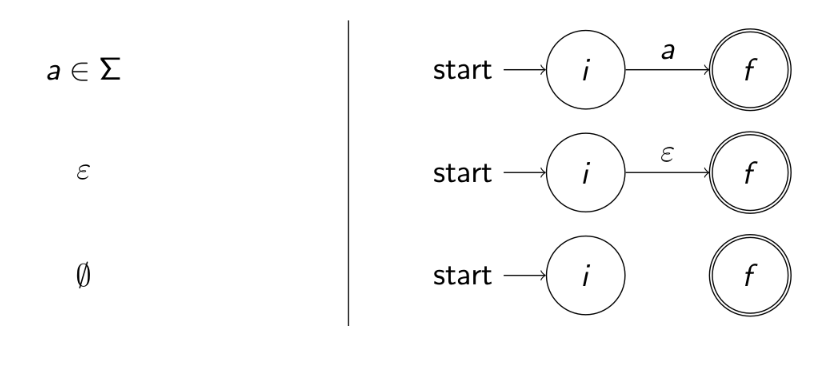
\includegraphics[scale=0.3]{Image4.png}
    \end{center}
    
    \item e$_{1}$+e$_{2}$ :
    \begin{center}
        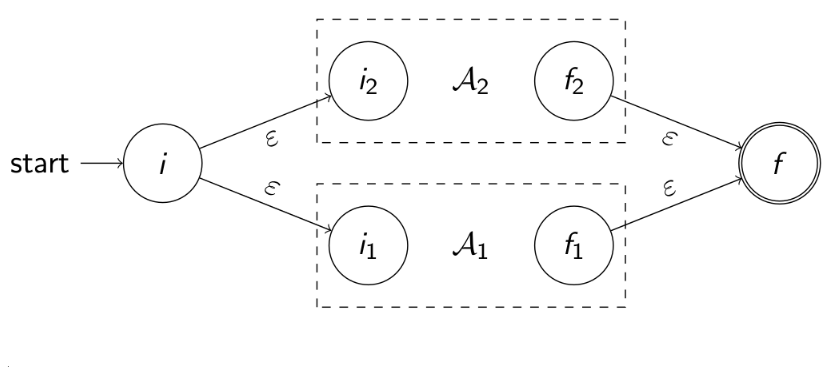
\includegraphics[scale=0.3]{Image5.png}
    \end{center}
    \item e$_{1}^{*}$ :
    \begin{center}
        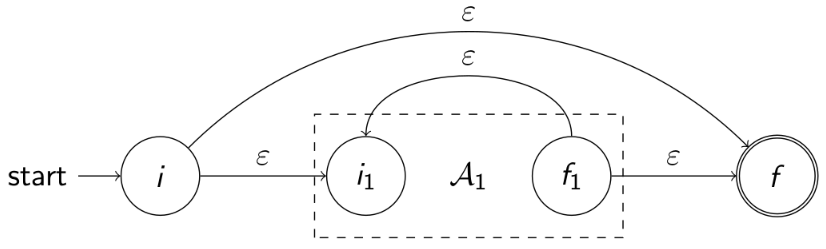
\includegraphics[scale=0.3]{Image6.png}
    \end{center}
    \item e$_{1}$ $\bullet$ e$_{2}$:
    \begin{center}
	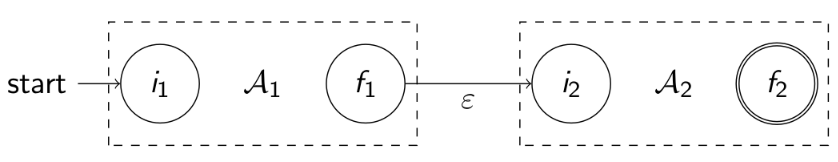
\includegraphics[scale=0.3]{Image7.png}
    \end{center}
    \item par exemple, à partir de la Regex a$^{*}$ + bc sur l'alphabet $\Sigma$ = \{a,b,c\} on obtient l'algorithme de Thompson suivant :
    \begin{center}
        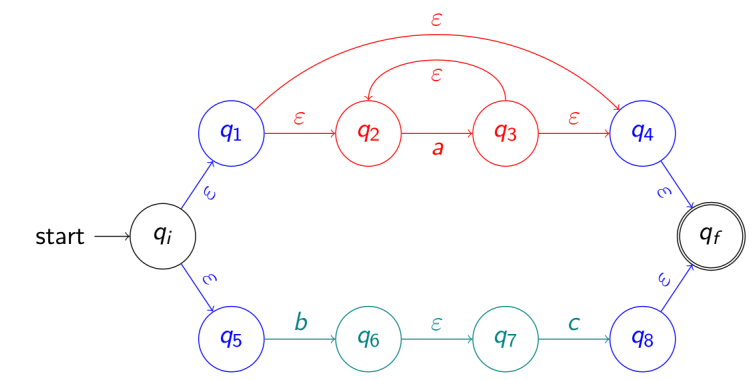
\includegraphics[scale=0.25]{Image8.png}
    \end{center}
    \item Soit e $\in$ Reg$_{\Sigma}$ une Regex et n le nombre d'occurences de \{$\varepsilon$,$\emptyset$,+,*, le nombre de lettres dans $\Sigma$\} (on exclue les parenthèses). Le nombre d'états est alors égale à 2n.

À partir de l'automate obtenu par l'algorithme de Thompson, on réduit à 0 les $\varepsilon$-transitions, en reliant les différents états nécessaires à l'état initial. Puis on modifie les derniers états en les modifiant par des états finaux.
\end{itemize}\newpage
\section{Simplification des $\varepsilon$-NFA}
C'est la partie du cours la plus compliquée, il y aura un certain nombre de termes techniques. Une bonne connaissance du cours vu jusqu'ici est absolument nécessaire à la compréhension de cette partie.\par
En reprenant le dernier automate obtenu (le dernier automate de la page précédente), on remarque qu'il y a beaucoup d'états qu'un automate déterministe aurait pu éviter. On va alors procéder à des \textit{éliminations arrière des $\varepsilon$-transitions} et des \textit{éliminations avant des $\varepsilon$-transitions}
\begin{itemize}
    \item élimination arrière des transitions spontanées :
    \begin{center}
        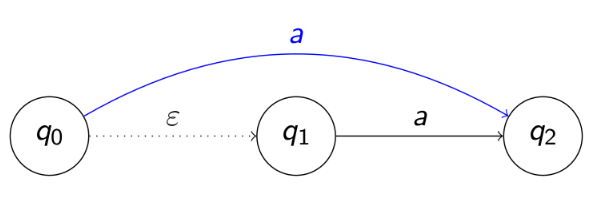
\includegraphics[scale=0.3]{Image9.png}
    \end{center}    
    \item élimination avant des transitions spontanées :
    \begin{center}
        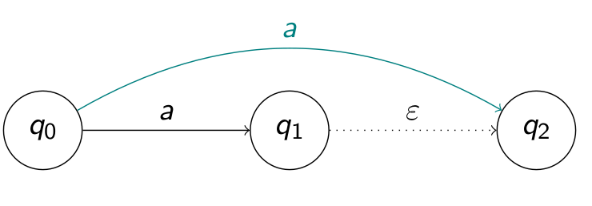
\includegraphics[scale=0.3]{Image10.png}
    \end{center}
\end{itemize}

On définit les $\varepsilon$-fermeture de la manière suivante :\newline\newline
\textbf{$\varepsilon$-fermeture d'un état :}
\begin{quote}
    La $\varepsilon$-fermeture $\varepsilon_{forward}^{A}$(q) d'un état q d'un automate $A$ est l'ensemble \{p$\in$Q$|$q$\xlongrightarrow{\text{epsilon}}$$_{A}^{*}$\}\newline
    Note : q $\in$ $\varepsilon_{forward}^{A}$ (q) car on peut atteindre q à partir de q en ne lisant rien du tout.
\end{quote}

Théorème :
\begin{quote}
    Si p $\in$ $\varepsilon_{forward}^{A}$(q) and r $\in$ $\varepsilon_{forward}^{A}$(p) alors r $\in$ $\varepsilon_{forward}^{A}$(q).\newline
    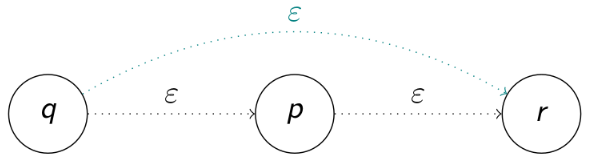
\includegraphics[scale=0.3]{Image11.png}
\end{quote}

\newpage
\section{Pruning et déterminisme}
\subsection{Pruning :}
Le NFA généré par l'algorithme de Thompson est compliqué, même avec les les suppressions arrières des $\varepsilon$-transistions. On va donc supprimer les états et transitions qui ne servent à rien.\newline\newline

\textbf{Utilité des états :} (soit $q$ un état de l'automate $A$)
\begin{quote}
    \begin{itemize}
        \item $q$ est dit \textit{accessible} s'il peut être atteint à partir d'un état initial
        \item $q$ est dit \textit{co-accessible} si à partir de q, on peut atteindre un état acceptant
        \item $q$ est dit \textit{utile} s'il est accessible \textbf{et} co-accessible.\newline
    \end{itemize}
    Si un état n'est ni accessible, ni co-accessible (donc par définition, pas utile), on dit qu'il est \textit{inutile}. 
\end{quote}

Ces états permettent d'introduire la notion de \textit{pruning} d'un automate.
\begin{quote}
    Soient $A$ un automate et $A'$ l'automate obtenu à partir de la suppression des états inutiles de $A$. On dit que $A$ est équivalent à $A'$.
\end{quote}

Ce théorème permet de donner l'algorithme de pruning:
\begin{enumerate}
    \item trouver les états accessibles (par un parcours profondeur ou largeur) depuis les états initiaux
    \item trouver les états co-accessibles (on "remonte" les flèches à partir des états acceptants)
    \item ne garder que les états accessibles et co-accessibles
\end{enumerate}
\begin{figure}
    \centering
    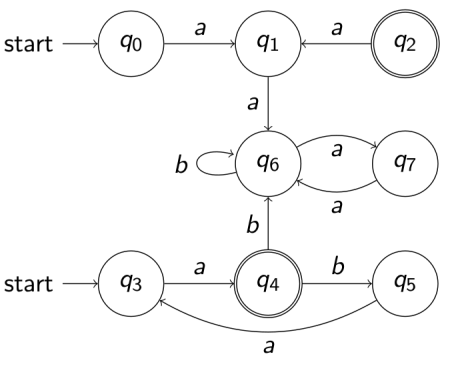
\includegraphics[scale=0.25]{Image12.png}
    \caption{automate $A$ sur l'alphabet $\Sigma$ = \{a,b\}}
\end{figure}
\begin{figure}
    \centering
    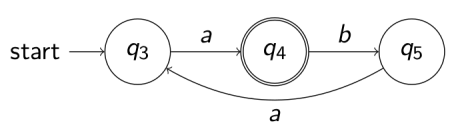
\includegraphics[scale=0.25]{Image13.png}
    \caption{automate $A'$ : A et A' sont équivalents}
\end{figure}
\newpage
\subsection{Déterminisme}
Petit rappel :
\begin{quote}
    Un NFA est dit déterministe si pour toute lettre $a$ et état $q$, il existe au plus une transition sortant de $q$ étiqueté par $a$.\newline
    Un NFA est dit complet si pour toute lettre $a$ et état $q$, il existe au moins une transition sortant de $q$ étiqueté par $a$.\newline
\end{quote}

Théorème
\begin{quote}
    $\forall$ $A$ NFA sur un alphabet $\Sigma$, $\exists$ un équivalent DFA $A'$ sur $\Sigma$ 
\end{quote}

\begin{figure}
    \centering
    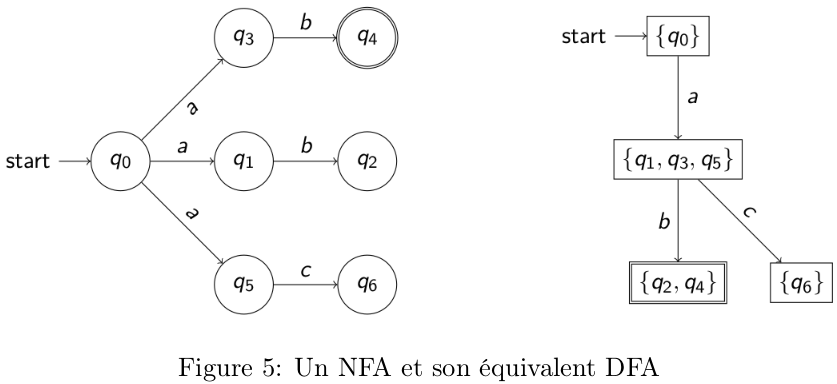
\includegraphics[scale=0.3]{Image14.png}
    \caption{Un NFA et son équivalent DFA}
\end{figure}
\newpage
\section{Lemme de pompage}
Théorème :
\begin{quote}
    Tous les langages rationnels sont décidables. La contraposée n'est pas toujours vraie.
\end{quote}

Lemme de pompage :
\begin{quote}
    Soit un langage rationnel L $\in$ Rat$_{\Sigma}$, il existe un niveau de pompage n$_{0}$ tel que pour tout mot w $\in$ L de longueur n$\geq$ n$_{0}$, il existe 3 mots x,y et z $\in$ $\Sigma^{*}$ tel que w = xyz, y $\neq$ $\varepsilon$, and $L$(xy$^{*}$z) $\subseteq$ L
\end{quote}

Théorème :
\begin{quote}
    Le langage L = \{a$^{n}$b$^{n}$ | n $\in$ $\mathbf{N}$\}, sur l'alphabet $\Sigma$=\{a,b\}, est décidable mais non rationnel.
\end{quote}

Un langage rationnel est reconnaissable par un algorithme qui utilise une quantité constante de données qui  ne dépend pas de la taille de l'input.

\section{Minimisation des automates}
Le déterminisme d'un automate d'une regex créé un nombre très élevé d'états. Dans l'ordre on a :
\begin{enumerate}
    \item expression régulère : n symboles
    \item $\varepsilon$-NFA : 2n états
    \item NFA : 2n états
    \item pruned NFA : $\leqslant$ 2n états
    \item DFA : $\leqslant$ 2$^{2n}$
\end{enumerate}

États indistinguables:
\begin{quote}
    Deux états $q_{1}$ et $q_{2}$ d'un DFA $A$ sont dits \textbf{indistinguables} si pour tout mot $w \in \Sigma^{*}$, de $q_{1}$, $A$ accepte $w$ ssi, depuis $q_{2}$, $A$ accepte $w$. On dit que $L_{q_{1}}$($A$) = $L_{q_{2}}$($A$).\newpage
    À partir de l'automate suivant :
    \begin{figure}[h]
        \centering
        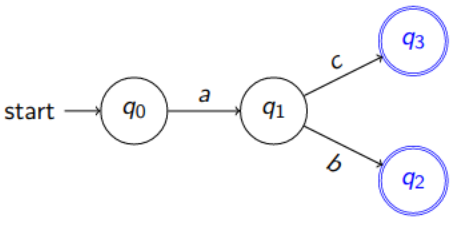
\includegraphics[scale=0.25]{Image15.png}
    \end{figure}
    on peut donner l'automate équivalent suivant :
    \begin{figure}[h]
        \centering
        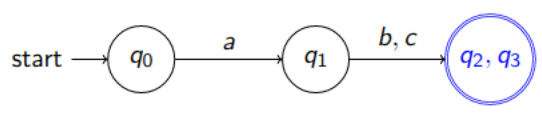
\includegraphics[scale=0.25]{Image16.png}
    \end{figure}
\end{quote}
Théorème de Myhil-Nerode :
\begin{quote}
    Soit un langage rationnel L, il existe un unique DFA $A$ avec un nombre minimal d'états (= au nombre d'états indistinguables de L) tel que $L$($A$) = L. On dit que cet automate est l'automate canonique de L.
\end{quote}

Ainsi, si deux états p$_{1}$ et p$_{2}$ d'un DFA $A$ sont indistinguables et p$_{1}$ $\rightarrow$ (a) q$_{1}$ et p$_{2}$ $\rightarrow$ (a) q$_{2}$, alors q$_{1}$ et q$_{2}$ sont eux aussi indistinguables.

(section à compléter, pas compris la fin du ppt)

\newpage
\section{Propriétés des langages rationnels}
\subsection{Algorithme de Brzozowski-McCluskey}
L'algorithme de Brzozowski-McCluskey consiste à transformer un automate avec plusieurs transitions à un automate avec un seul état initial, un seul état final et une seule transition entre les deux états. Cette transition doit contenir l'expression régulière qui doit être égale au langage initial. L'état initial ne doit pas avoir de transitions entrantes et l'état final ne doit pas avoir de transitions sortantes. Au final, l'automate doit avoir exactement cette structure :
\begin{figure}[h]
    \centering
    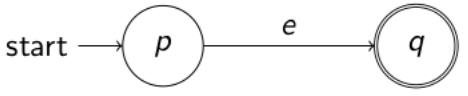
\includegraphics[scale=0.5]{Image17.png}
    \caption{e doit être équivalent au langage initial}
\end{figure}

Cet algorithme a pour conséquence le théorème suivant :
\begin{quote}
    Soit un automate $A$ sur un alphabet $\Sigma$, il existe une expression régulière e $\in$ Reg$_{\Sigma}$ tel que $L(A)$ = $L$(e), c'est-à-dire que e est \textbf{équivalent} à $A$.
\end{quote}

\subsection{Stabilité des propriétés des langages rationnels}
On considère un langage L rationnel (L$\in$Rat$_{\Sigma}$):
\begin{itemize}
    \item $\overline{L} \in$ Rat$_{\Sigma}$.
    \item Pref(L), Fact(L) et Suff(L) $\in$Rat$_{\Sigma}$
    \item L$^{R}$ (langage miroir) $\in$Rat$_{\Sigma}$
    \item Si L$_{1}$, L$_{2}$ $\in$Rat$_{\Sigma}$, alors L$_{1}$$\cap$L$_{2}$$\in$Rat$_{\Sigma}$
    \item on peut savoir si L = $\oslash$ ou non (si on peut accéder à un état acceptant depuis l'état initial)
    \item soit L'$\in$Rat$_{\Sigma}$, on peut savoir si L = L' ou non
\end{itemize}

\section{Précisions à partir des questions de QCM}
\begin{itemize}
    \item Un langage peut être infini mais un alphabet est nécessairement fini.
	\item Un langage récursif n'est pas défini par récurrence.
	\item Le facteur d'un langage peut être le préfixe du suffixe et le suffixe du préfixe d'un langage.
	\item L'étoile de Kleene d'un langage fini peut être infini.
	\item Les langages rationnels sont stables par étoile de Kleene, concaténation et union.
	\item Tout langage rationnel vérifie le lemme de pompage mais tout langage qui vérifie le lemme de pompage n'est pas rationnel.
	\item L'inclusion ne préserve pas la rationalité.
	\item Il n'existe pas de mot à longueur infini.
    \item Soit L un langage ne contenant pas $\varepsilon$. $\varepsilon$ appartient à L* mais pas à L$^{+}$.
\end{itemize}
\end{document}
